\documentclass{article}

\usepackage{url} % Tidy web links
\usepackage{microtype} % 'Improved' typesetting
\usepackage{parskip} % Adds white space between paragraphs
\usepackage[super]{natbib} % Citations using superscript
\usepackage[a4paper, left=1.5cm, right=1.5cm, top=1.5cm, bottom=2.0cm]{geometry}
\usepackage{longtable,booktabs}  % For tables
\usepackage{caption} % For figure and table captions
\usepackage{graphicx} % Adds more functionality to graphics for inclusion of figures
\usepackage{lineno} % Allows use of \linenumbers to add line numbers 
\usepackage[toc,page]{appendix}
\usepackage[utf8]{inputenc}
\frenchspacing % No double spacing between sentences
\linespread{1.2} % Set linespace
\usepackage{authblk} % For author formatting
\usepackage{lmodern} % A scalable font - avoids erros due to non-sclabale fonts
\usepackage{subcaption} % Allows use of subfigures
\DeclareUnicodeCharacter{2060}{\nolinebreak} % Prevent unicode (U+2060) error on local complile
\usepackage{cclicenses} % For creative commons license
\usepackage{xcolor} % for coloured text
\usepackage{xurl} %for url but with more flexible linebreaking
\usepackage[hybrid]{markdown}

\renewcommand{\thefootnote}{\alph{footnote}} % Use letters for footnotes


% Choose your own colour
\usepackage{color}
\newcommand{\mjanote}[2][\textcolor{red}{\dagger}]{\textcolor{red}{$#1$}\marginpar{\color{red}\raggedright\tiny$#1$ #2}}
\newcommand{\mjaFIXME}[1]{\textcolor{red}{[\textbf{FIXME} \textsl{#1}]}}
\newcommand{\kpnote}[2][\textcolor{magenta}{\dagger}]{\textcolor{magenta}{$#1$}\marginpar{\color{magenta}\raggedright\tiny$#1$ #2}}
\newcommand{\kpFIXME}[1]{\textcolor{magenta}{[\textbf{FIXME} \textsl{#1}]}}

\hbadness=1000000 % Turn off \hbox badness warnings

\begin{document}

% Rewrite this title to include dementia

\title{STOKE-IMPACT: Understanding the impact of clinical practice variation on patient outcomes using explainable machine learning coupled with clinical trial emulation and causal inference studies. A study using national clinical audit data.}
\author{} % Hide author
\date{} % Hide date
\maketitle
\vspace{-20mm}

%\section*{Summary}


The focus of our team's work is on using explainable machine learning, clinical pathway simulation, and geographic modelling, applied to national clinical audit data to identify between-hospital variation in clinical decision-making and processes, and understanding the impact of that variation on patients. Our work is in collaboration with the Sentinel National Stroke Audit Programme, and focuses mostly on the emergency stroke pathway, but is applicable across other clinical areas.

We would like to enhance our methodology by adding causal analysis methods to support the explainable machine learning. This would include a literature review, but we expect it to include methods such as:

\begin{markdown}
* Clinical Trial Emulation
* Bayesian networks
* Causal Inference Machine Learning
* Instrumental Variable Analysis
\end{markdown}

As no method is perfect we wish to be able to develop a range of causal models to allow triangulation of results, and identify the best methods to incorporate into our integrated modelling and data science approach. This will allow us to propose and refine causal structures for discussion with clinicians. The novelty of our work is to combine state-of-the art modelling and data sceince techniques with large-scale data sets to address issues of variation in clinical care.

This enhanced methodology has potential immediate uses that will benefit patients and the NHS:

* We are working with the national stroke audit to help build machine learning into their national audit outputs, especially on unnecessary variation in use of clot-bust treatments in stroke. We are working with NHS-England to provide this analysis to new communities of practice in stroke. We have identified that a majority of the variation comes from differences in clinical decision-making rather than in differences in local patient populations. This is a NIHR-funded project \footnote{https://fundingawards.nihr.ac.uk/award/NIHR134326}. The methodological development will enhance the breadth and depth of that work, helping to identify and isolate causal relationships. Improving use of clot-busting drugs will benefit patients (and should reduce inpatient length of stay).

* We are working on stroke projects focussing on the pre-hospital pathway \footnote{https://fundingawards.nihr.ac.uk/award/NIHR202361} and the use of mobile stroke units \footnote{https://fundingawards.nihr.ac.uk/award/NIHR153982 (page due to go live)}. The methodological development above will add value to these, and other similar, projects. For example, it has previously been assumed that outcome from hemorrhagic stroke (the 20\% of strokes that are caused by a bleed rather than a clot) is independent of ambulance travel time, but some recent clinical trials on taking stroke patients further, to a hospital with more capabilities for stokes caused by clots, have suggested this may not be true. Using methods such as clinical trial emulation and our large database of stroke data we will have the potential to enhance our pre-hospital stroke care model to better model outcomes of haemorrhagic strokes with alternative pre-hospital pathways.

During this project we will hold stakeholder workshops, to obtain feedback on the work. This will use our existing stakeholder network across thr Sentinel Stroke National Audit, Integrated Stroke Delivery Networks (ISDN) and Integrated Care Systems (ICS). We will also hold regular meetings with our stroke Patient and Carer Involvement group.

In addition to development of the methodology, this project will be used to develop the skills and capabilities of Kerry Pearn (co-PI) who will lead the project with assistance from Michael Allen (Co-PI). The stroke modelling and data science team is a stable team, funded by research grants and NHS-contracted work, and the techniques and skills developed here will find long-term use and benefit.


\begin{figure}[htbp]
\centering
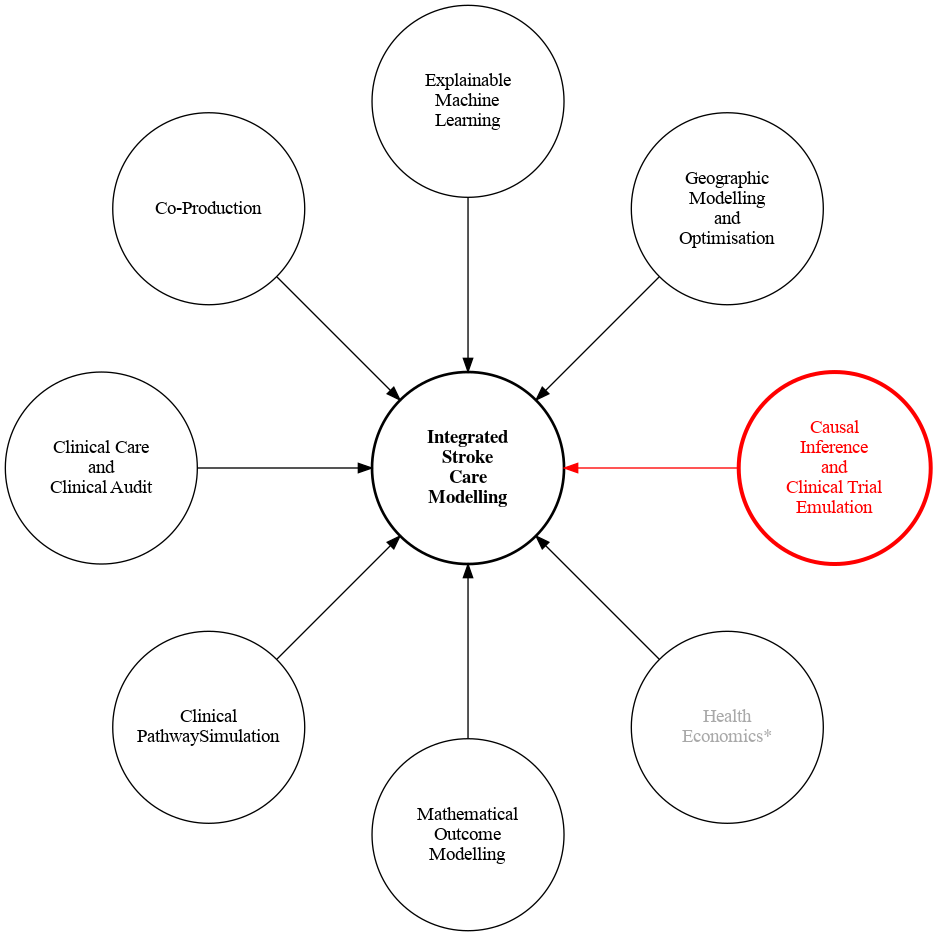
\includegraphics[width=0.6\textwidth]{./images/skills}
\caption{How planned methodology development (red) fits in with existing team skills (black) or collaborative work (grey). All methods are fully pubslished with open code.}.
\label{fig:expertise}
\end{figure}

\section*{Plain English Summary}

The focus of our team's work is on using explainable machine learning, clinical pathway simulation, and geographic modelling, applied to national clinical audit data to identify between-hospital variation in clinical decision-making and processes, and understanding the impact of that variation on patients and on the use of health service resources. Our work is in collaboration with the Sentinel National Stroke Audit Programme, and focuses mostly on the emergency stroke pathway, but is applicable across other clinical areas.

In our work we uncover potential causes of between-hospital variation. For example, in the use of clot-busting medication (\textit{thrombolysis}) in stroke, the majority of the large between-hospital variation in use of these drugs appears to come from differences in decision-making and in-hospital processes, rather than from differences in the characteristics of the patients attending each hospital. Another example is that appears early use of these clot-busting drugs reduces the risk of death even in mild strokes, but late use can increase the risk of death. These are important observations that may be used to advocate for change in clinical practice. Though our models attempt to isolate the effects of different factors, we would like to use multiple different methods to strengthen the \textit{cause-and-effect} conclusions from our current models. This will help rule out our current observations being coincidence (for example, if early use of clot-busting drugs is linked to a reduction in death, can we be sure this isn't just because the patients receiving treatment earlier have characteristics that make them less likely to die anyway?). We wish, for example, to confirm that early use of thrombolysis is actually causing the observed reduction in death. To do this we would use methods known as \textit{causal inference analysis}.

When using data that has been collected in routine clinical practice, no method is perfect for confirming a cause-and-effect, but by incorporating multiple methods into our analysis we wish to test our observations from our machine learning as much as possible. Example methods that might be used include \textit{target trial emulation} (where the patient set is restricted to those that have been through clinical trials in a similar area of study), or \textit{matching} where matched pairs of patients are found that are very similar apart from the one characteristic that we think may be important.

Adding methods that more directly investigate cause-and-effect will substantially strengthen our suite of tools. We have recently added \textit{explainability} to our machine-learning models (so that we can see what led to any particular prediction the model made). Adding stronger cause-and-effect analysis would help test our models further and build more trust in conclusions and recommendations made. 

The work will find immediate use in the various stroke modelling projects we undertake with the national stroke audit and with national and regional NHS organisations. During this project we will hold stakeholder workshops, to help develop the work so it is understable by, and useful for, stakeholders. This will use our existing stakeholder network across the Sentinel Stroke National Audit including the newly established NHS-England \textit{communities of practice of thrombolysis}, which bring together stroke teams with differing use of clot-busting drugs. We will also regularly involve patients and carers in discussing the work - our experience is that this very significantly helps test our knowledge on the models, and helps us to develop much clearer communication of the models and the results.

In addition to development of the methodology, this project will be used to develop the skills and capabilities of Kerry Pearn (co-PI) who will lead the project with assistance from Michael Allen (Co-PI). The stroke modelling and data science team is a stable team, funded by research grants and NHS-contracted work, and the techniques and skills developed here will find long-term use and benefit.
%\section{Bid Info}

\url{https://www.nihr.ac.uk/funding/rfpb-under-represented-disciplines-and-specialisms-highlight-notice-methodologists/33231}

\begin{markdown}

* Call opens – 17 May 2023    \item Expression of Interest - (500 words) 16 August 2023 at 1pm
* Close call – 13 September at 1pm
* Stage 1 outcome – December 2023
* Stage 2 call close - end of January 2024
* Stage 2 outcome – May 2024
* Start - September 2024?

## What does RfPB cover?

* Research into the provision and use of NHS services.
* Effectiveness and cost effectiveness evaluations of interventions.
* Research that examines the resource use of alternative means for healthcare delivery.
* Feasibility research to support applications for major awards to other funders.
* Development and refining of new interventions, scales or outcome measures.
*  Research to explore the potential for improving patient health and wellbeing through needs assessments, methods development and exploratory studies.
* Evidence synthesis and systematic reviews
\end{markdown}

%\begin{markdown}
# Background
\end{markdown}

%\section{Method development}


%\markdownInput{sections/9_stuff_to_inlcude.md}

\end{document}

